\documentclass[a4paper]{article}
\usepackage[utf8]{inputenc}
\usepackage[czech]{babel}
\usepackage[T1]{fontenc}

\usepackage[pdftex]{graphicx}
\usepackage{ifpdf}
\usepackage{hyperref}

\title{gScrabble -- Programátorská dokumentace}

\author{Ondrej Profant}

\date{\today}

\ifpdf
\hypersetup{
	pdfauthor={Ondrej Profant},
	pdftitle={gScrabble -- Uzivatelská prirucka},
}
\fi

\begin{document}

\tableofcontents	

\section{Použité nástroje}
Program je psán v jazyce C\# (verze 4) a využívá knihoven GTK\#. 
Pro vývoj bylo použito vývojové prostředí MonoDevelop (2.6) a distribuoaný systém správy verzí GIT.
Pro tvorbu grafiky Inkscape (0.48), externí dokumentace je psaná v LaTeXu. Vyvíjeno na Ubuntu 11.04.

\section{Zdrojové kódy}
Příkazem: \texttt{git clone git://github.com/Kedrigern/scrabble.git} získáte celý projekt. 
Soubor s koncovkou \texttt{sln} lze otevřít v MonoDevelop, které vám zobrazí celou strukturu zdrojových kódů velmi přehledně, vypadá přibližně takto:

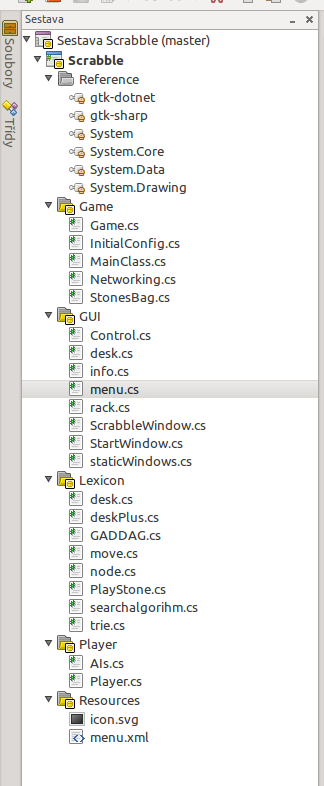
\includegraphics[scale=0.5]{pic/monodevelop-project.png}

Struktura rozdělení zdrojových kódů snad mluví sama za sebe. Většina důležitých tříd a funkcí je komentovaná přímo v kódu. 

\end{document}
